%%%%%%%%%%%%%%%%%%%%%%%%%%%%%%%%%%%%%%%%%%%%%%%%%%%%%%%%%%%%%%%%%%%%%%%%%%%%
%% Author template for Decision Analysis (deca)
%% Mirko Janc, Ph.D., INFORMS, mirko.janc@informs.org
%% ver. 0.95, December 2010
%%%%%%%%%%%%%%%%%%%%%%%%%%%%%%%%%%%%%%%%%%%%%%%%%%%%%%%%%%%%%%%%%%%%%%%%%%%%
%\documentclass[deca,blindrev]{informs3}
\documentclass[deca,blindrev]{informs3} % current default for manuscript submission

\OneAndAHalfSpacedXI % current default line spacing
%%\OneAndAHalfSpacedXII
%%\DoubleSpacedXII
%%\DoubleSpacedXI

% If hyperref is used, dvi-to-ps driver of choice must be declared as
%   an additional option to the \documentclass. For example
%\documentclass[dvips,deca]{informs3}      % if dvips is used
%\documentclass[dvipsone,deca]{informs3}   % if dvipsone is used, etc.

% Private macros here (check that there is no clash with the style)

% Natbib setup for author-year style
\usepackage{natbib}
 \bibpunct[, ]{(}{)}{,}{a}{}{,}%
 \def\bibfont{\small}%
 \def\bibsep{\smallskipamount}%
 \def\bibhang{24pt}%
 \def\newblock{\ }%
 \def\BIBand{and}%

%% Setup of theorem styles. Outcomment only one. 
%% Preferred default is the first option.
\TheoremsNumberedThrough     % Preferred (Theorem 1, Lemma 1, Theorem 2)
%\TheoremsNumberedByChapter  % (Theorem 1.1, Lema 1.1, Theorem 1.2)

%% Setup of the equation numbering system. Outcomment only one.
%% Preferred default is the first option.
\EquationsNumberedThrough    % Default: (1), (2), ...
%\EquationsNumberedBySection % (1.1), (1.2), ...

% In the reviewing and copyediting stage enter the manuscript number.
%\MANUSCRIPTNO{} % When the article is logged in and DOI assigned to it,
                 %   this manuscript number is no longer necessary

%%%%%%%%%%%%%%%%
\begin{document}
%%%%%%%%%%%%%%%%

% Outcomment only when entries are known. Otherwise leave as is and 
%   default values will be used.
%\setcounter{page}{1}
%\VOLUME{00}%
%\NO{0}%
%\MONTH{Xxxxx}% (month or a similar seasonal id)
%\YEAR{0000}% e.g., 2005
%\FIRSTPAGE{000}%
%\LASTPAGE{000}%
%\SHORTYEAR{00}% shortened year (two-digit)
%\ISSUE{0000} %
%\LONGFIRSTPAGE{0001} %
%\DOI{10.1287/xxxx.0000.0000}%

% Author's names for the running heads
% Sample depending on the number of authors;
\RUNAUTHOR{Duan}
% \RUNAUTHOR{Jones and Wilson}
% \RUNAUTHOR{Jones, Miller, and Wilson}
% \RUNAUTHOR{Jones et al.} % for four or more authors
% Enter authors following the given pattern:
%\RUNAUTHOR{}

% Title or shortened title suitable for running heads. Sample:
 \RUNTITLE{Bias and Accuracy of ML Models}
% Enter the (shortened) title:
%\RUNTITLE{}

% Full title. Sample:
\TITLE{Exposing Model Bias in Machine Learning: Revisiting the Boy Who Cried Wolf in the Context of Phishing Detection}
% Enter the full title:
%\TITLE{}

% Block of authors and their affiliations starts here:
% NOTE: Authors with same affiliation, if the order of authors allows, 
%   should be entered in ONE field, separated by a comma. 
%   \EMAIL field can be repeated if more than one author
\ARTICLEAUTHORS{%
\AUTHOR{C.J.Duan}
\AFF{Dulun Consulting Group, \EMAIL{research@dulun.com}, \URL{http://www.dulun.com}}
%\AUTHOR{Author2}
%\AFF{Author2 affiliation, \EMAIL{}, \URL{}}
% Enter all authorsdulun.com
} % end of the block

\ABSTRACT{%
Grown out of the quest for artificial intelligence (AI), machine learning (ML) is today's most active field across disciplines with sharp increase in applications ranging from criminology to fraud detection and to biometrics. ML and statistics both emphasize model estimation / training and thus share the inescapable Type 1 and 2 errors. Extending the concept of statistical errors into the domain of ML, we devise a ground-breaking pH scale-like ratio and intend it as a litmus test indicator of ML model bias completely masked by the popular performance criterion of accuracy. Using publicly available phishing dataset, we conduct experiments on a series of classification models and consequently unravel the significant cost implications of models with varying levels of bias. Based on the results, we recommend practitioners exercise human judgment and match their own risk tolerance profile with the bias ratio associated with each ML model in order to guard against potential unintended adverse effects.% Enter your abstract
}%

% Sample
%\KEYWORDS{deterministic inventory theory; infinite linear programming duality; 
%  existence of optimal policies; semi-Markov decision process; cyclic schedule}
	
% Fill in data. If unknown, outcomment the field
\KEYWORDS{machine learning, Type 1 and 2 errors, bias ratio, phishing websites classification}
%\HISTORY{submitted on April 4, 2018}

\maketitle
%%%%%%%%%%%%%%%%%%%%%%%%%%%%%%%%%%%%%%%%%%%%%%%%%%%%%%%%%%%%%%%%%%%%%%

% Samples of sectioning (and labeling) in DECA
% NOTE: (1) \section and \subsection do NOT end with a period
%       (2) \subsubsection and lower need end punctuation
%       (3) capitalization is as shown (title style).
%
%\section{Introduction.}\label{intro} %%1.
%\subsection{Duality and the Classical EOQ Problem.}\label{class-EOQ} %% 1.1.
%\subsection{Outline.}\label{outline1} %% 1.2.
%\subsubsection{Cyclic Schedules for the General Deterministic SMDP.}
%  \label{cyclic-schedules} %% 1.2.1
%\section{Problem Description.}\label{problemdescription} %% 2.

% Text of your paper here

\section{Introduction}

Aesop's fable, the “The Boy who Cried Wolf,” is about a young shepherd boy found his life dull in the pasture as he sat on the hillside tending his master’s sheep. To amuse himself, he ran toward the village shouting at the top of his voice, "Wolf! Wolf! The Wolf is chasing the sheep!". The villagers dropped their work and rushed up the hill to help the boy scare the wolf away. But upon their arrival, they found no wolf and only the grinning face of the shepherd boy. "Don't cry 'wolf', when there's no wolf!" The
grumbling villagers told the boy and returned to their village. A few days later, the boy felt bored and yell out again, "Wolf! Wolf! The wolf is chasing my sheep!" To his wicked delight, he viewed the villagers dash up the hill and fall for his trick gain. The villagers sternly warned "Don't cry 'wolf' when there is NO wolf!". Later, he saw a real wolf prowling about his herd. In terror, he leaped to his feet and sang out as loudly as he could, "Wolf! Wolf!". To no avail, the villagers thought he was trying to repeat his foolish game, so they stay away. At sunset, everyone wondered why the shepherd boy hadn't returned to the village with their sheep. They went up the hill and found him weeping. The price the village paid is costly: the killing of a great many of the flock.

At the end of the story, an old man comforted the boy. “If you tell too many lies, no one believes you when you tell the truth. The moral message the tale conveys is that liars are not trustworthy even when they are telling the truth. Undoubtedly, the shepherd boy was not even close to a pure rational decision maker, perhaps a naughty one. Considering his maturity level and working environment, are we being too harsh on the young boy entrusted with the task of guarding the village's most valuable asset? \cite{doi:10.1175/1520-0434(2004)019<0391:TBWCWR>2.0.CO;2} delineate the classical tale in a decision-making matrix as shown in table \ref{tab1}. Based on their cost-loss analysis,  the villagers in the tale were unprepared to tolerate a reasonably high  false-alarm rate (cries of “Wolf!” when there is no wolf looming). As revealed by our ensuing investigation, even machine learning (ML) models trained on large data sets are not immune from sounding false alarms.

\begin{table}
\TABLE
{The Villagers’ Benefit and Cost Matrix \label{tab1}}
{\begin{tabular}{ccc}
\hline 
\up \down & \multicolumn{2}{c}{Perception }\\
\hline 
\up \down Reality & Wolf - Yes & Wolf - No\\
\hline 
\up Wolf & Respond and Rescue & Stay Put \\
\down -Yes&  6 villagers for 1 hr {@}  \$10 $h^{-1}$ & Killing of 3 sheep {@}\$200 each\\
\hline 
\up Wolf & Respond and Disappointed & No Action and No Harm\\
\down  -No&  6 villagers for 1 hr {@}  \$10 $h^{-1}$ & \$ 0\\
\hline
\end{tabular}}
{Adapted from \cite{doi:10.1175/1520-0434(2004)019<0391:TBWCWR>2.0.CO;2} }
\end{table}

Our research was motivated by what we observed as a slight disconnect between the computing side (predictive accuracy) and statistical side (model bias) of ML. ML should induce  more objective and evidence-based decision-making, since machines are supposedly free from human prejudice. However, as revealed in the work of \cite{Caliskan2017},  machine learning (language processing) can acquire stereotyped biases from textual data reflecting everyday human culture. As noted by \cite{Kleinberg2017}, applied ML work typically focuses on the link between data and prediction, while paying less attention to the prediction$\to$decision link. The limitations of any  model trained on real data  necessitates human experts' judgment back into the decision-making processes - for the worse or the better \citep{lewis2016undoing}.

%As a demonstration effort, one major point to mention at the start is that our project did not focus on any testable hypotheses per se.
Andrew Ng, Google Brain founder, once stated that ``Simply downloading and `applying'  open-source software to your data won't work. AI needs to be customized to your business context and data'' \citep{ng2016artificial}.
Answering the call for more human-centered AI \citep{FF2018}, our study was undertaken with four overall goals:

\begin{henumerate}
\item To alert the decision analysis  community to the prevalence and perils of model bias in ML.
% increasing popularity of AI-powered  machine decision making (MDM) and automation, which pose to render vast swaths of the working professionals literally redundant.

\item To propose and formulate a litmus ratio (akin to the pH scale in chemistry) for the assessment of model bias common in ML.
\item To demonstrate empirically the trade-off between model accuracy and bias that  requires human judgment and stringent regulation in order to to minimize total combined  disutility
\item To illustrate  how human adopters of ML models can use our proposed litmus ratio to diagnose and mitigate bias implicit in ML.
 
%To put “old wine” (statistical errors) into new bottles (machine learning framework) and examine how the decision-making environment (phishing detection) influences model selection, which subsequently leas to the minimization of expected disutility - the opposite of maximization of expected utility .
\end{henumerate}

The paper proceeds as follows. In the Related Works section, we describe phishing detection, which serves as the context of our experiments. Also explicated in that same section are classification algorithms in ML, as well as widely adopted metrics used to appraise ML algorithm performance. Amid the Proposed Litmus Ratio section, we formulate a unique ratio for the purpose of assessing ML model bias and derive the total cost function with accuracy and bias as the two input factors. In the Data, Models  and Empirical Analyses section, we first introduce the Phishing dataset, and develop a large set of models based on the dataset.  Then, we present the results acquired from out experiments. In the Implications section, we discuss how to match a model's litmus ratio to the risk toleration profile of the decision-maker circumvented by the surrounding environment. In the Concluding Remarks section, we spotlight the importance of human intelligence in the face of wide-spreading AI. 


\section{Related Works }

\subsection{Classification using ML Algorithms}

\cite{mitchell1997machine}  defined machine learning as, ``a  computer program is said to learn from experience ‘E’ with respect to some class of task ‘T’ and performance measure ‘P’, if its performance in task ‘T’, as measured by ‘P’, improves with experience E'' (p. 2). Machine learning is the manifestation of statistical learning (statistics) algorithms implemented via software (computing) applications. The concept of machine learning has been in existence for decades. But it was only until recently that machine learning began to see its explosive applications to huge quantities of data attributed to the confluence of powerful computers, cheap storage of data, and vast availability of analytical opportunities, among others. Being a subfield of artificial intelligence, machine learning rests on the paradigm that algorithms can learn from data and reason with data \citep{rao2013handbook}. Based on the desired outcome and the type of input available for training the system, machine learning algorithms generally fall into either supervised or unsupervised learning.  In the former, a trainer carefully selects examples for the learner and the learner must sort those examples into categories specified by the trainer, whereas in the latter the learner is given little or no instruction on the learning task and the goal is to find underlying regularities \citep{cottrell2006new}.

There exists considerable overlap between statistics and machine learning. Both fields focus on studying generalization from data (model building). However, statistics, inferential statistics in particular, makes generalization (prediction) about the unknown population parameters (parameter estimation) based on often small sample. Machine learning, on the other hand, relies heavily on the predictive accuracy of models, while ignoring largely checking of models and assumptions. In addition, terminology employed in machine learning is different from that used by statisticians. In machine learning, a target or outcome is called a label, while in statistics it is referred to as dependent variable (DV). In statistics, an input predictor is called an independent variable, whereas it is denoted as a feature in machine learning.  

In a classification ML problem, the focal algorithm  is  presented  a training data sample of n observations on a categorical (class) variable (label) Y and a set of $m$ predictor variables X \{$X_1, X_2, \cdots, X_m\}$  (features) that are either categorical or continuous. The goal of the learning process is then  to find a model predicting Y values from those of X \citep{Loh2011}. Classification tree methods typically partition recursively the training dataset one $X_i$ at a time to achieve minimal  impurity (measure of misclassification). 

Originally proposed by \cite{kass1980exploratory}, the acronym CHAID stands for Chi-squared Automated Interaction Detection. It aims to detect interactions between categorized variables of a data set, one of which is the outcome variable or label. CHAID is a classification tree algorithm to construct a non-binary decision tree, where two or more branches can attach to a single node.  Because the CHAID algorithm will often effectively build many multi-way frequency tables (e.g., when classifying a categorical response variable with many classes, based on categorical predictors with many classes), small sample size may not yield optimum prediction. The algorithm is implemented based on recursive partitioning and is purported to maximize the significance of a chi-squared statistic for cross-tabulations between the dependent variable and the predictors at each partition. The data are partitioned into mutually exclusive, exhaustive subsets that best describe the outcome variable. Multiway splits are used by default.  It is non-parametric and  quite proficient in handling large dataset.
 
\subsection{Phishing Detection}
Phishing is defined as a social engineering technique where the aggressor pretends to be a trustworthy entity in attempt to gain sensitive information (e.g. usernames, password, credit card credentials) from the victim \citep{Jagatic2007}. In the cyber-attack, fraudulent website con users into disclosing sensitive and/or confidential information to the attacker by impersonating to be a legitimate website in an automated fashion.  These types of communications are commonly accomplished through emails that point users to phishing websites through which phishers gather information in question.  Bank and credit card details, password, and personal identification number are few examples that interest phishers frequently collect users’ credentials \citep{jakobsson2006phishing}

Phishing websites has been a persistent threat and it has been a major concern of cyber security.  According to the report published by Anti Phishing Working Group (APWG) in December 2016, the unique phishing sites detected only in 3rd quarter of 2016 are 364,424. The most common methods of phishing involve some forms of technical deception designed to make a link in an email (and the spoofed website it leads to) appear to belong to the spoofed organization. 

In reviewing the applied ML research on phishing websites classification,   \cite{Mohammad2015a} highlighted three steps in the intelligent  heuristics  based  anti-phishing approach.  First, a set of discriminating features (presence of special symbols, and URL length, etc.) are collected. Then,  a ML model is trained to separate phishing links from legitimate ones based on the selected link features. Finally, the tuned model is applied in real world setting to recognize phishing attempts.  So far, the most advanced ML model we found is the Self-Structuring Neural Network developped by \cite{7727750}. Their proposed iSSNN classifier was found to show competitive results against other ``off-the-shelf'' algorithms, including Logistic Regression (LR), Decision Tree (C4.5), Bayesian Network (BN),and  Feed Forward Neural Network (FFNN).
The latest observed results from \cite{10.1007/978-981-10-5699-4_50}  showed that tree-based classifiers, such as Random tree,  provide maximum accuracy with comparison to other counterparts.

 



\subsection{Evaluation of classification  ML Algorithms}

In assessment of (binary) classification  ML algorithm performance, the predicted  values and actual label values  are often cross-tabulated into  a typical confusion matrix (CM) contained in  table \ref{tab2}. Our acquaintance with null hypothesis  significance  testing (NHST) easily alludes us to Type 1 ($\alpha$) and  Type 2 error ($\beta$). Type 1 error,  also known as “false positive”, is the false rejection of a null hypothesis when it is true. Plainly speaking, it arises when we are detecting a difference when there is none. Type 2  error, also known as "false negative", is the error of not rejecting a null hypothesis when the null hypothesis is the false state of reality. In other words, it occurs when we are failing to detect a difference when the difference in fact exists. As described below, all common metrics in the assessment of ML classifying models are derived from such CM.

Accuracy is the most intuitive performance measure of a ML classification model  and it is simply the ratio of correctly predicted observation (both phishing and legitimate) to the total observations in the test dataset.

\begin{equation}
Accuracy = \frac {TP+TN}{TP+FP+TN+FN}
\end{equation}

Precision, also known as PPV (Positive Predictive Value) is the rate of correctly predicted positive labels to the total predicted positive observations.  It is calculated as:

\begin{equation}
Precision = \frac {TP}{TP+FP}
\end{equation}

Recall, also known as Sensitivity or True Positive Rate (TPR), is  is the ratio of correctly predicted positive observations to the all observations in actual ``+'' class:

\begin{equation}
Recall = \frac {TP}{TP+FN}
\end{equation} 

Specificity, also known as True Negative Rate (TNR),  is the ratio of correctly predicted ``-'' observations to the all observations in actual``-'' class:

\begin{equation}
Specificity = \frac {TN}{FP+TN}
\end{equation}

F1 score is the weighted average or harmonic mean of Precision (P) and Recall (R). Thus, it takes both false positives and false negatives into account, as shown in equation (5).

\begin{equation}
F1 = \frac {2*P*R}{P + R}
\end{equation}
\\
After intensive review of metrics deployed in assessment of ML classifiers, we found no metrics involve only FP and FN in definition. Inspired by this obvious absence of bias measuring metrics, we, in the next section, take the first step and attempt to  formulate a simple Litmus ratio that can be applied in evaluating ML model bias.
  


\begin{table}
\TABLE
{Sample Confusion Matrix \label{tab2}}
{\begin{tabular}{ccc}
\hline 
\up \down & \multicolumn{2}{c}{Predicted Value}\\
\hline 
\up \down Actual & + & -\\
\hline 
\up + & True Positive (TP) & False Negative (FN) \\
% \down & Time and Efforts well spent & Loss of Assets\\
\hline 
\up - & False Positive (FP) & True Negative (TN)\\
%\down  & Waste of Time and Efforts & Zero Cost\\
\hline
\end{tabular}}
{Adapted from \cite{7727750} }
\end{table}




\section {The Proposed Litmus Ratio}

We now formally define the Litmus ratio $\tau = \frac{\alpha}{\beta}$, where $\alpha$  is the total number of false positive cases misclassified and $\beta$  is the false negative counterpart within the  test data set of size N. If $\varLambda$  is the accuracy of the corresponding ML model, we can then establish

\begin{equation}
1 - \varLambda = \frac {\alpha + \beta}{N}
\end{equation}

Substitute $\alpha$ with $\tau\beta$, we arrive at:

\begin{equation}
1 - \varLambda = \beta\frac {1+\tau}{N}\Rightarrow \beta = N*\frac {1-\varLambda}{1+\tau}
\end{equation}

With $C_{FP}$ and   $C_{FN}$ represent unit cost (negative) of FP and FN error respectively, we can easily calculate the total cost of misclassifications ($\varGamma$) as:
 
%\begin{equation}
%\begin{cases}
%FN = \frac{N*E}{1+\iota}\\
 %FP = \frac{N*E\iota}{1+\iota}
%\end{cases}
%\end{equation}
 
\begin{equation}
\varGamma =  N*\frac {(1-\varLambda)\tau}{(1+\tau)}*C_{FP} + N*\frac {1-\varLambda}{(1+\tau)}*C_{FN}
\end{equation}
For simplicity of presentation, we use $k=\frac{C_{FP}}{C_{FN}}$ and further reduce  equation 3 to :

\begin{equation}
\varGamma = \alpha*C_{FP} + \beta*C_{FN} =  N*(1-\varLambda)*C_{FN}*\frac{(k\tau+1)}{(1+\tau)}
\end{equation}

Consider a special case of $ k=1$  (neutral decision-making environment), we have  $\varGamma =  N*(1-\varLambda)*C_{FN}$, which indicates that the best model is the one with the highest accuracy only and bias is canceled out.

%Also under  relatively static decision-making circumstances, we can assume away $N, C_{FN} $ and better understand the interplay between accuracy and bias. 
%\begin{equation}
%\varGamma^{\prime} = (1-\varLambda)*\frac{k\tau+1}{(1+\tau)}
%\end{equation}

%Suppose we face a set of models with the same level of accuracy, we can further reduce the above equation to

%\begin{equation}
%\varGamma^{\prime} = \frac{k\tau^\prime + 1-k}{\tau^\prime} = k + \frac{1 - k}{\tau^\prime}
%\end{equation} 

Without any further calculus work, we can see the close ties between model characteristics and the cost characteristics of the corresponding decision-making environment, represented by $\tau (\tau^\prime), \varLambda$ and k respectively. The purpose of next section is to empirically demonstrate the ($\varLambda - \tau$) -  k links, which can be applied to the screening of ML model candidates.


\section{Data, Models  and Empirical Analyses}

The Phishing Websites Dataset \citep{Mohammad2015} , used in this work, is available online at the UCI Repository \citep{Dua2017}. The dataset has been
used in several works that either propose new  or evaluate existing techniques for phishing website classification \citep{7727750, Mohammad2012, Mohammad2013, Mohammad2015a}. It contains data from 11055  websites  labeled into  two major classes (-1 for phishing and 1 for legitimate). Of the 11055 observations, 44\% take the value of -1 (phishing) and 56\% take the value of 1 (legitimate).  Each instance contains 30 features / attributes, which fall into four broad categories. Feature 1 through 12 belong to the Address Bar Based Features category Abnormal Based Features occupy the next 6 features. Feature 19 - 23 are bundled into the HTML and JavaScript Based Features, while Domain Based Features claim the remaining 7 attributes. All 30 features have been  preprocessed into either dichotomous (-1 for phishing positive, 1 for phishing  negative) or trichotomous (-1, 1, and 0 for phishing neutral).  

Customarily, we split the whole dataset into 80\% for training and 20\% (size of 2211) for testing. We carried  out experimental analyses on the CRAN-R platform \citep{R2013}.  In the first phase, we feed the whole training dataset of size 8844  into the CHAID algorithm implemented by the R-Forge Project Team \citep{chaid}, while restricting the variety of features involved in model training. 


%=================================
\begin{table}
\TABLE
{Performance Results \label{tab3}}
{\begin{tabular}{clcc}
\hline 
\up \down Model &  Features &  $\varLambda$  & $\tau$ \\
\hline
\up \down 1  &01 - 12  &  90\% & 0.78 \\
\up \down 2 &  13 - 18 &  88\% & 0.24 \\
\up \down 3  &  19 - 23 &  57\% & 0.01 \\
\up \down 4  &  24 - 30 &  73\% & 0.57 \\
\up \down 5  &  01 - 30  &  95\% & 1.27 \\
\hline
\end{tabular}}
{Models differ in features included }
\end{table}
%================================

We summarized the performance  of each of the five models  assessed on the test dataset in table \ref{tab3}. The full model with all 30 features outperformed the other 4 sub-models by the margins ranging from 5\% to 38\% in terms of accuracy. Model 3, which considers only  the HTML and JavaScript Based Features, yielded the lowest accuracy and extremest bias. Like regression in statistical analysis, we observe that individual (categories of) features do not contribute equally to model accuracy. It is also noteworthy that the full model (model 5) not only improves accuracy to the highest level, but also shifts the bias from the  $<1$ side to the $>1$  side. It seemingly  confirms that  in ML,  the more objective the data and the larger the data set, the less possibility of distortion, as noted by \cite{Rosso2015}.

In the second phase of our empirical analyses, we created 1,000 models, which  consider the same set of  30 available features, but differs mainly  in the records contained in the training data. Via iterative re-sampling, 
we created 1,000 different samples of size of  7075 (80\% of 8844) from  the original training dataset and fed each sample into the CHAID algorithm.  The 1,000 models are plotted in Figure \ref{fig1} along the dimensions of accuracy and bias. This arrangement allows us to investigate the impact of various accuracy-bias combinations on the total cost of misclassification ($\varGamma$).
 
%================================
\begin{figure}
\FIGURE
{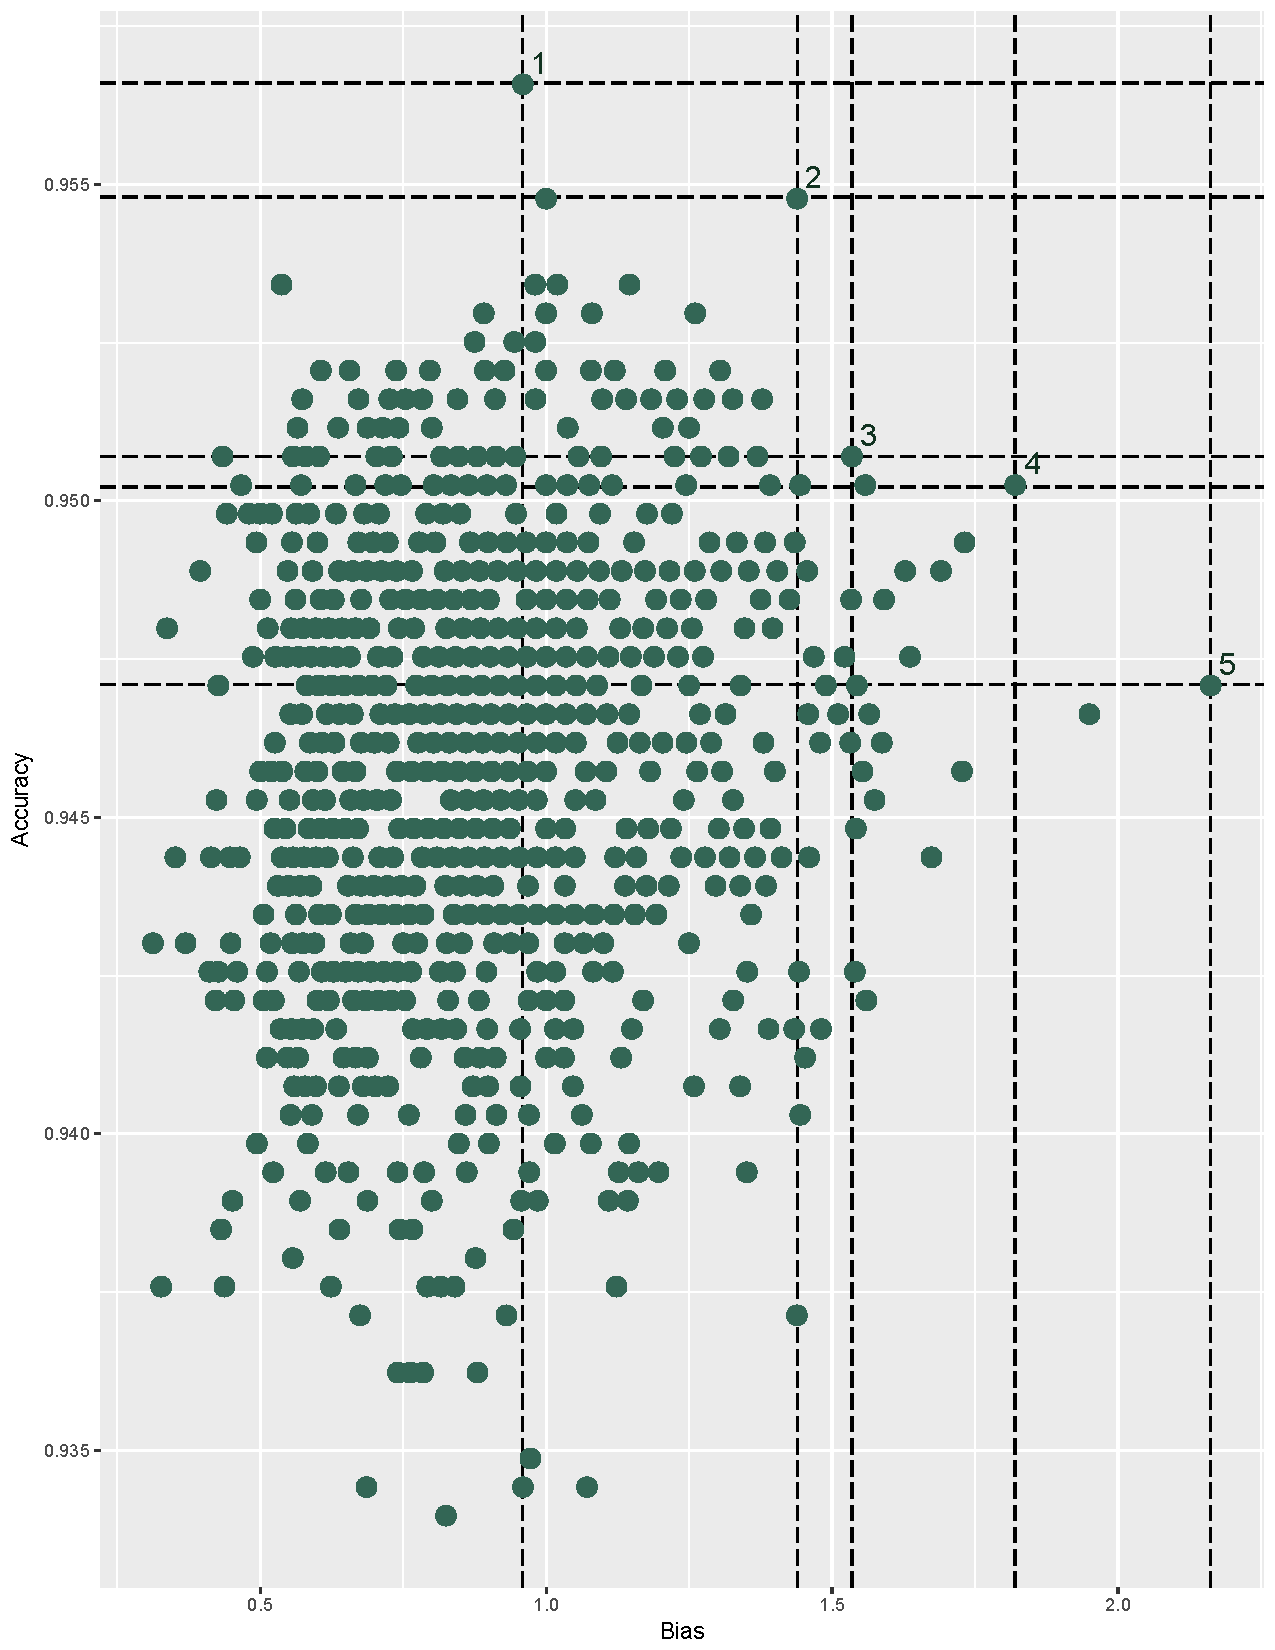
\includegraphics[width=0.65\linewidth]{Rplot04.pdf}}
{Bias - Accuracy Scatter Plot \label{fig1}}
{each dot represents one model with unique parameterization }
\end{figure}
%=============================== 

The context of phishing detection resembles the situation faced by the villagers  in the opening fable, in that $C_{FN}$ far outweighs $C_{FP}$. For  illustration purposes,  we set k = 1/10 and computed the $\varGamma$ for each of the five models in the top-right quadrant. Surprisingly, we noticed in Table \ref{tab4} that the best model with the lowest $\varGamma$ of 44.49  is model \#5, which has the worst accuracy of 94.7\% among the five models studied. The model with the highest accuracy of 95.7\% (model \#1) yielded the worst total cost figure of 53.66. The worsened predictive accuracy is well compensated by the right-shifting bias factor.  
    
%================================
\begin{table}
\TABLE
{Accuracy and Bias Tradeoff  \label{tab4}}
{\begin{tabular}{cccccc}
\hline 
\up \down Model &  N  &  $\varLambda$  & k & $\tau$  & $\varGamma$ \\
\hline
\up \down 1&2211&0.957&1/10&0.96& 53.66\\
\up \down 2&2211&0.955&1/10&1.44& 46.86\\
\up \down 3&2211&0.951&1/10&1.54& 49.60\\
\up \down 4&2211&0.950&1/10&1.82& 46.13\\
\up \down 5&2211&0.947&1/10&2.16& 44.49\\
\hline
\end{tabular}}
{All models with the same set of features

Total Costs are in units of $C_{FN}, k=\frac {C_{FP}}{C_{FN}}$}
\end{table}
%================================

\section{Implications}

The opening fable is supposed to teach young readers a moral lesson on integrity and honesty by showing the severe negative damage to the society caused by the  shepherd boy’s lying. Put the moral lesson aside, we can base on the experiments described above and draw alternative lessons from the imprudent decision making by the villagers in the same story.  When they handed over the custody of the sheep herd to the young shepherd boy, the villagers as decision-makers should have known upfront that the young boy is error-prone. More specifically, he tends to make false alarms about wolfs’ attack because he is not assumed to possess the capability to fend off the attacks himself. With zero possibility of false negatives (type II error), the villagers should foresee that only false alarm is left to him to make. Further, responding to the boy\textsc{\char13}s crying wolf costs only a couple of hours of delay of thier planned  farm work, which is no way comparable to the loss of several sheep to lupine attacks. Given the skewed  $\frac{C_{FP}}{C_{FN}}=1/10$  ratio, smart decision makers should respond to every alarms regardless of their potential spuriousness. Maybe after responding to a few rounds of no-wolf false alarms, the villagers as asset owners should delegate the task of safeguarding their herd to a more mature and capable shepherd. In the context of ML, we can imagine a flying drone equipped with a video camera might do a better job to protect the herd and even entertain the boy. 

Unfortunately, such a decision-making lesson is not confined to characters in stories. As demonstrated with our experiments, even machine learning models trained on large real life datasets bear significant behavioral resemblance to the young shepherd boy in the tale. Without the necessary human guidance and even human interference, the seemingly almighty machine intelligence can lead to disastrous  consequences. Demonstrative in nature, our work is desired to unmask model bias and to develop mitigating measures that practitioners can readily implement to reap maximal benefits from ML. 

Because we utilized the same hold-out dataset to test all models, we are afforded the opportunity to unravel the familiar type I and II errors in statistics in the context of machine learning. Completely masked by the overall misclassification rate, type I and II errors take on significantly different meanings in the evaluation of machine learning models. Regarding labeling phishing websites, a type I error means a legitimate website is wrongly put on blacklist. Consequently, this overestimation of the potential risk posed by the candidate website will induce wasted resources, most of which are largely opportunity costs (the extra hour spent finding alternative websites to get the original job done). On the other hand, underestimation of potential phishing threat will definitely deal identity theft and resultant financial loss and psychological stress to the victim. If we assume an individual’s identity and fanatical safety is one of the most critical assets and the extra time wasted on searching for alternative websites due to false alarms can be reasonably expressed in hourly wages, the  contextual cost ratio of $k=\frac{C_{FP}}{C_{FN}}$ should be even more skewed than 1/10. Obviously, the small k ratio tilts heavily toward underestimation of risk and hence necessitates models with significantly low type II error rate, which translates into model bias ratio $\tau \approx \frac{1}{k} > 10$. As shown in table \ref{tab4}, our best  model  only slightly favors $\alpha$  with a $\tau$ ratio of 2.2. Our analysis indicates that the 1\% decrease in accuracy is well offset by the doubling of the bias ratio in terms of the combined adverse impact on cost.  

 It is also clear from the results that we in practice need to search for best possible solutions that minimize total disutility governed by both overall error rate and the relative distribution of Type 1 and 2 errors. Consider, for instance, the life-threatening situation faced by actress Angelina Jolie. Female carriers of a BRCA1 / BRCA2 genetic mutation must decide whether to undergo BM (bilateral mastectomy) and / or BSO (bilateral salpingo-oophorectomy), both of which are invasive with serious side effects and possible severe complications \citep{Joliemay14}. Relative to the FN risk (actual high cancer risk without preventive bilateral mastectomies), the daunting FP (actual low cancer risk with decision to undergo BM/BSO) costs in this case can, in no small measure, dominate the minds of most BRCA1/2 carriers. It was the ``Jolie Effect'' that tipped the scale and  doubled rates of preventive bilateral mastectomies \citep{evans2015longer}. As \cite{Nohdurft2017} argued, women exhibit varying degrees of preference about the feasibility and timing of  preventive bilateral mastectomies due to individual differences in perceived risk of cancer associated with BRCA1/2. In this scenario, the differing estimation of FP costs and  FN risk from instance to instance can further complicates the winnowing process of model selection because our analysis of total costs is aggregate in nature.  
 
To end this section, we reiterate that the selection of machine learning models must cater to the risk-tolerance profile of the human decision-maker. The perceived cost-and-risk distribution is in turn influenced and to some extent  dictated by the specific circumstances  surrounding the decision-maker. In other  words, the process of  data$\to$prediction$\to$decision needs to be viewed holistically and well tuned under human guidance.



\section {Concluding Remarks}

George Box, ``one of the great statistical minds of the 20th century'',  made the famous quote - ``all models are wrong, but some are useful'' \citep[p. 424]{box1987empirical}.  The aphorism today still shines a somewhat colder light on the much hyped and feared might of machine learning and AI. Decision analysis is  based on the maximum expected utility (MEU) action axiom, the basic proposition of which states that  human beings purposely utilize means in order to pursue  desired ends. To make high quality decisions, a decision-making agent (partnership between man and machine)  must have a sense of the association between various actions and the likelihood of different outcomes, as well as the desirability of each such outcome. Correspondingly, they represent prediction (from input features to output labels) and judgment (assign values to the expected utility of models derived). On the one hand,  latest advances in AI vastly  reduced the cost of prediction. On the other hand, AI also substantially raised the value of human judgment \citep{Agrawal2018}. To this end, we put forward our own version of Box's apothegm -    ``All models are biased, some are agreeably  preferred''


%======================================================
% Acknowledgments here
\ACKNOWLEDGMENT{%
% Enter the text of acknowledgments here
}% Leave this (end of acknowledgment)


% Appendix here
% Options are (1) APPENDIX (with or without general title) or 
%             (2) APPENDICES (if it has more than one unrelated sections)
% Outcomment the appropriate case if necessary
%
% \begin{APPENDIX}{<Title of the Appendix>}
% \end{APPENDIX}
%
%   or 
%
% \begin{APPENDICES}
% \section{<Title of Section A>}
% \section{<Title of Section B>}
% etc
% \end{APPENDICES}
\newpage

%==========================================================
%\begin{table}
%\TABLE
%{The Villagers’ Benefit and Cost Matrix \label{tab1}}
%{\begin{tabular}{ccc}
%\hline 
%\up \down & \multicolumn{2}{c}{Perception }\\
%\hline 
%\up \down Reality & Wolf - Yes & Wolf - No\\
%\hline 
%\up Wolf & Respond and Rescue & Stay Put \\
 %\down -Yes& Time and Efforts well spent & Loss of Assets\\
%\hline 
%\up Wolf & Opportunity Cost & No Harm\\
%\down  -No& Waste of Time and Efforts & Zero Cost\\
%\hline
%\end{tabular}}
%{Adapted from \cite{doi:10.1175/1520-0434(2004)019<0391:TBWCWR>2.0.CO;2} }
%\end{table}
%================
%\begin{table}
%\TABLE
%{Sample Confusion Matrix \label{tab2}}
%{\begin{tabular}{ccc}
%\hline 
%\up \down & \multicolumn{2}{c}{Predicted Value}\\
%\hline 
%\up \down Actual & + & -\\
%\hline 
%\up + & True Positive (TP) & False Negative (FN) \\
% \down & Time and Efforts well spent & Loss of Assets\\
%\hline 
%\up - & False Positive (FP) & True Negative (TN)\\
%\down  & Waste of Time and Efforts & Zero Cost\\
%\hline
%\end{tabular}}
%{Adapted from \cite{7727750} }
%\end{table}
%==================================
%\begin{table}
%\TABLE
%{Performance Results \label{tab3}}
%{\begin{tabular}{clcc}
%\hline 
%\up \down Model &  Features &  Precision & Litmus Ratio \\
%\hline
%\up \down 1  &01 - 12  &  90\% & 0.78 \\
%\up \down 2 &  13 - 18 &  88\% & 0.24 \\
%\up \down 3  &  19 - 23 &  57\% & 0.01 \\
%\up \down 4  &  24 - 30 &  73\% & 0.57 \\
%\up \down 5  &  01 - 30  &  95\% & 1.27 \\
%\hline
%\end{tabular}}
%{Models differ in features included }
%\end{table}
%==================================
\newpage
%\begin{figure}
%\FIGURE
%{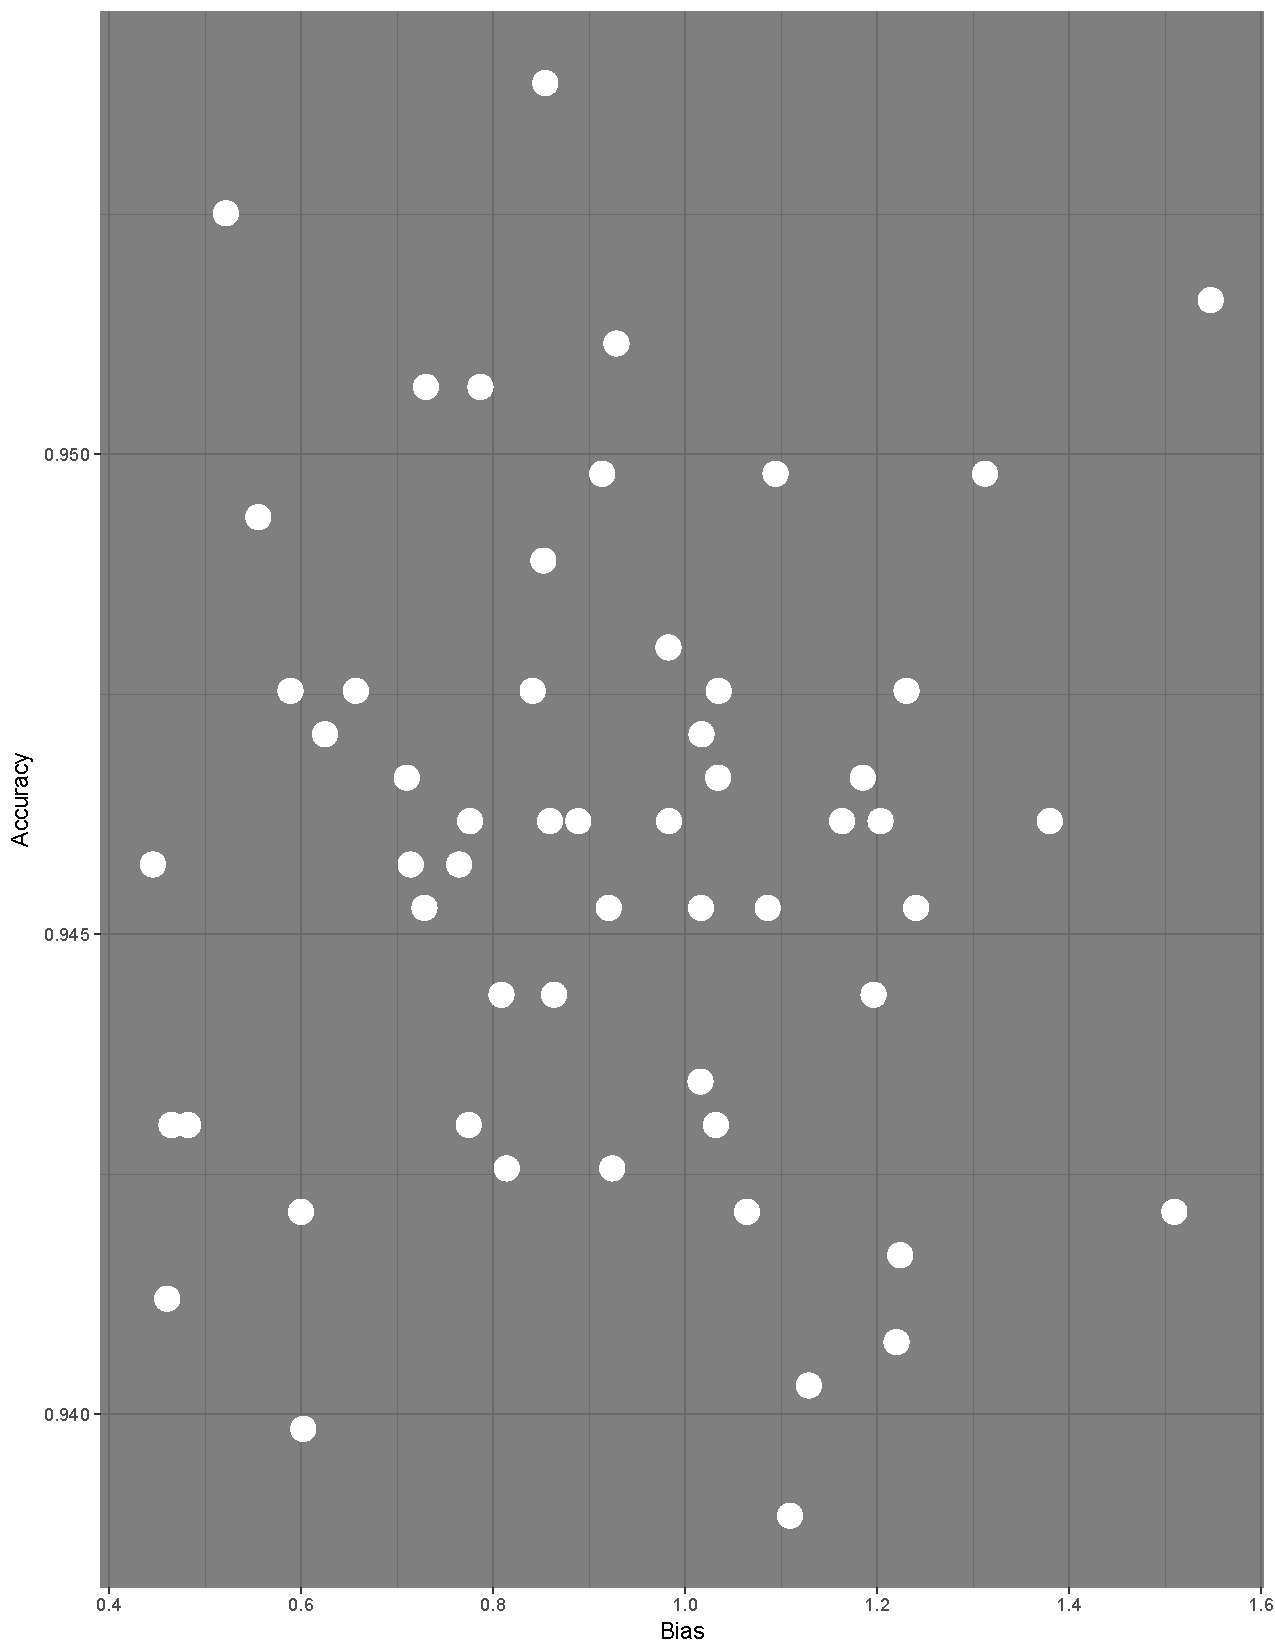
\includegraphics[width=0.5\linewidth]{Rplot.pdf}}
%{Figure Caption. \label{fig1}}
%{Text of Notes}
%\end{figure}


\newpage
% References here (outcomment the appropriate case) 

% CASE 1: BiBTeX used to constantly update the references 
%   (while the paper is being writduanten).
\bibliographystyle{informs2014} % outcomment this and next line in Case 1
\bibliography{duan} % if more than one, comma separated

% CASE 2: BiBTeX used to generate mypaper.bbl (to be further fine tuned)
%\input{mypaper.bbl} % outcomment this line in Case 2

\end{document}


